\documentclass[11pt,border=5pt]{standalone}
\usepackage{fontspec}
\setmainfont{cmunrm.otf}[BoldFont=cmunbx.otf,ItalicFont=cmunti.otf,BoldItalicFont=cmunbi.otf]
\usepackage{amsmath}
\usepackage{unicode-math}
\setmathfont{NewCMMath-Regular.otf}
\usepackage{tikz}
\usetikzlibrary{arrows.meta,patterns,angles,quotes}
\begin{document}
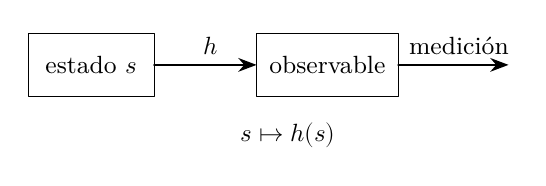
\begin{tikzpicture}[>=Stealth,font=\small,line cap=round,line join=round]
\draw[fill=white] (-2.8,-0.4) rectangle (-1.2,0.4);
\node at (-2,0) {estado $s$};
\draw[fill=white] (0.09999999999999998,-0.4) rectangle (1.9,0.4);
\node at (1,0) {observable};
\draw[->,thick] (-1.2,0) -- (0.1,0) node[pos=0.55,above] {$h$};
\draw[->,thick] (1.9,0) -- (3.3,0) node[pos=0.55,above] {medición};
\node at (0.5,-0.9) {$s\mapsto h(s)$};

\end{tikzpicture}
\end{document}
